\documentclass{standalone} % DO NOT CHANGE THIS
\usepackage{tikz}
\usepackage[utf8]{inputenc}
\usepackage{graphicx}
\usepackage{times}
\usepackage{amssymb}
\usepackage{xcolor}
\usetikzlibrary[arrows.meta, positioning,math, calc, shapes.geometric,intersections, fit, backgrounds, decorations.pathmorphing]

\definecolor{post}{rgb}{1., 0.25, 0.25}

\begin{document}

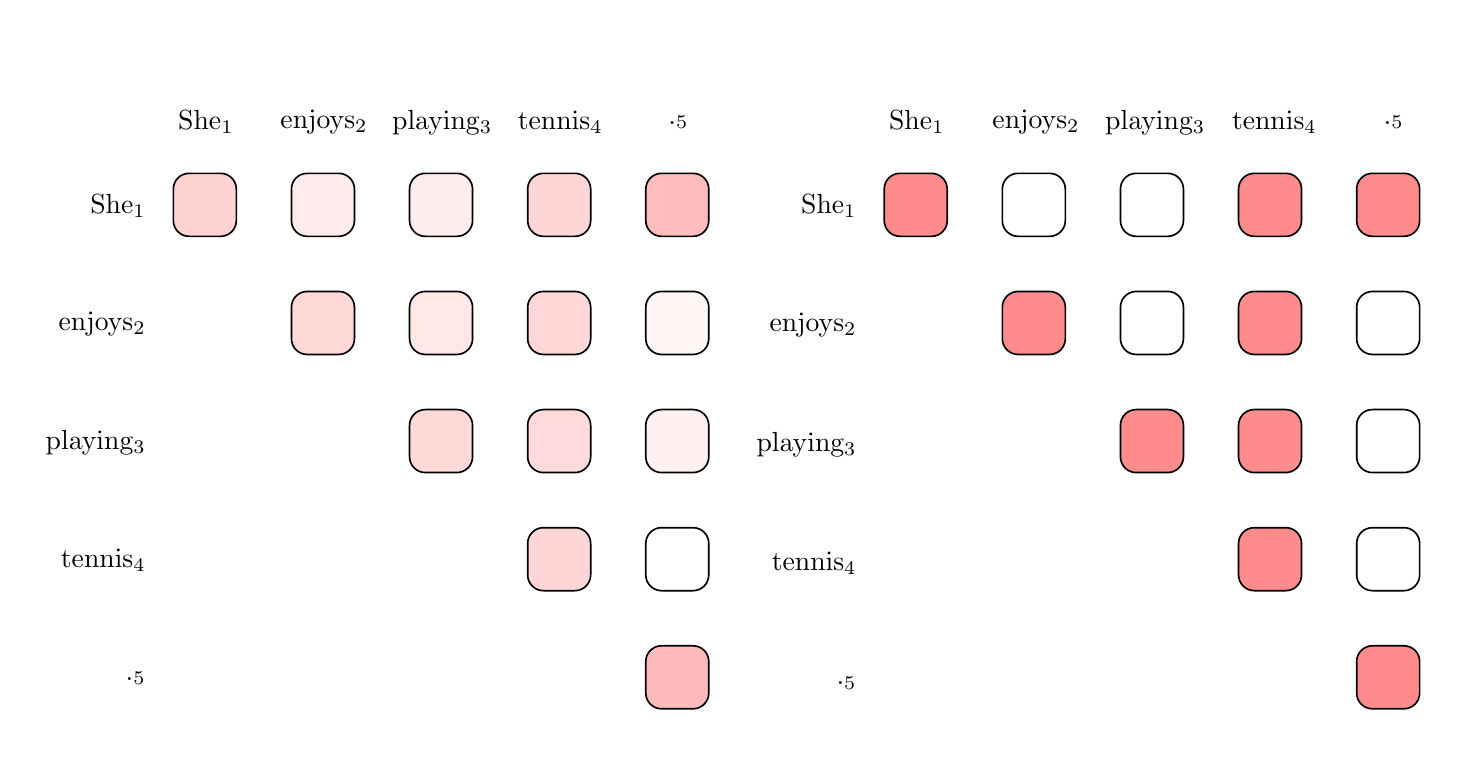
\begin{tikzpicture}[
    word/.style={
            minimum width=1.5cm,
            minimum height=1.5cm,
            inner sep=0pt,
            text width=1.5cm,
            % draw=black
        },
    red filled/.style={
            fill={rgb,255:red,238; green,63; blue,77},
        },
    blue filled/.style={
            fill={rgb,255:red,17; green,101; blue,154},,
        },
    red connect/.style={
            draw={rgb,255:red,238; green,63; blue,77},
            shorten >= 1pt,
            shorten <= 1pt,
            semithick
        },
    blue connect/.style={
            draw={rgb,255:red,17; green,101; blue,154},
            shorten >= 1pt,
            shorten <= 1pt,
            semithick
        },
    connect/.style={
            shorten >= -0.5pt,
            shorten <= 1pt,
        },
    chart/.style={
            minimum size=0.8cm,
            rounded corners=2mm,
            draw=gray,
            fill opacity=50,
            thick
            % thin,
        },
    dep arrow/.style={
    arrows={-Latex[round,length=6pt,width=3.5pt]},
    semithick
    },
    post score/.style={
            fill=red!50,
            draw={rgb,255:red,238; green,89; blue,100},
        },
    neg score/.style={
            draw={rgb,255:red,93; green,157; blue,177},
        },
    ]
    \centering

    \node [word] [anchor=south west] (w00) {};
    \node [word] [anchor=north, align=right] (w001) at ($(w00.south) - (0, 1.5cm*0)$) {She$_1$};
    \node [word] [anchor=north, align=right] (w002) at ($(w00.south) - (0, 1.5cm*1)$) {enjoys$_2$};
    \node [word] [anchor=north, align=right] (w003) at ($(w00.south) - (0, 1.5cm*2)$) {playing$_3$};
    \node [word] [anchor=north, align=right] (w004) at ($(w00.south) - (0, 1.5cm*3)$) {tennis$_4$};
    \node [word] [anchor=north, align=right] (w005) at ($(w00.south) - (0, 1.5cm*4)$) {.$_5$};
    \node [word] [anchor=south west, text centered, minimum height=0.6cm] (w010) at ($(w00.south east) + (1.5cm*0, 0)$) {She$_1$};
    \node [word] [anchor=south west, text centered, minimum height=0.6cm] (w020) at ($(w00.south east) + (1.5cm*1, 0)$) {enjoys$_2$};
    \node [word] [anchor=south west, text centered, minimum height=0.6cm] (w030) at ($(w00.south east) + (1.5cm*2, 0)$) {playing$_3$};
    \node [word] [anchor=south west, text centered, minimum height=0.6cm] (w040) at ($(w00.south east) + (1.5cm*3, 0)$) {tennis$_4$};
    \node [word] [anchor=south west, text centered, minimum height=0.6cm] (w050) at ($(w00.south east) + (1.5cm*4, 0)$) {.$_5$};

    % [[[0.0, 12.420832633972168, -10.051758766174316, -11.28689956665039, 9.164031028747559, 30.973827362060547], [0.0, 0.0, 6.660987377166748, -6.668295860290527, 7.720921993255615, -19.139789581298828], [0.0, 0.0, 0.0, 7.533620834350586, 4.98905086517334, -15.147298812866211], [0.0, 0.0, 0.0, 0.0, 9.548113822937012, -26.86586570739746], [0.0, 0.0, 0.0, 0.0, 0.0, 32.30168533325195], [0.0, 0.0, 0.0, 0.0, 0.0, 0.0]]]
    \foreach \y [count=\n] in {
            { 39., 17., 16., 36., 58.},
            {  0., 34., 20., 35.,  8.},
            {  0.,  0., 34., 32., 12.},
            {  0.,  0.,  0., 36.,  0.},
            {  0.,  0.,  0.,  0., 59.},
        } {
            \foreach \x [count=\m] in \y {
                \pgfmathsetmacro{\c}{\x*0.6}
                \ifnum\m<\n
                    % \node [circle,draw=gray, densely dashed ,semithick]  (w\x\y) at ($(w00.base) + (1.5cm*\m,-1.5cm*\n)$) {};
                \else
                    \node [chart,draw=black,fill=post!\c, semithick,inner sep=0pt]  (w\x\y) at ($(w00.base) + (1.5cm*\m,-1.5cm*\n)$) {};
                \fi
            }
        }


    \node [word] [anchor=south west] (w10) at (w050.south east) {};
    \node [word] [anchor=north, align=right] (w101) at (w10.south) {She$_1$};
    \node [word] [anchor=north, align=right] (w102) at (w101.south) {enjoys$_2$};
    \node [word] [anchor=north, align=right] (w103) at (w102.south) {playing$_3$};
    \node [word] [anchor=north, align=right] (w104) at (w103.south) {tennis$_4$};
    \node [word] [anchor=north, align=right] (w105) at (w104.south) {.$_5$};
    \node [word] [anchor=south west, text centered, minimum height=0.6cm] (w110) at (w10.south east) {She$_1$};
    \node [word] [anchor=west, text centered, minimum height=0.6cm] (w120) at (w110.east) {enjoys$_2$};
    \node [word] [anchor=west, text centered, minimum height=0.6cm] (w130) at (w120.east) {playing$_3$};
    \node [word] [anchor=west, text centered, minimum height=0.6cm] (w140) at (w130.east) {tennis$_4$};
    \node [word] [anchor=west, text centered, minimum height=0.6cm] (w150) at (w140.east) {.$_5$};

    % [[0.9998871088027954, 0.9999997615814209, 2.309833462277311e-07, 4.712777865734097e-07, 0.9999985694885254, 1.0], [0.036094143986701965, 0.651378333568573, 0.9999834299087524, 0.00015601464838255197, 0.9999146461486816, 2.5146931204034217e-09], [0.28686389327049255, 0.9329245090484619, 0.9889302849769592, 0.9999260902404785, 0.9979616403579712, 6.486852299758539e-08], [0.023861374706029892, 0.9903542995452881, 0.9446026682853699, 0.9999885559082031, 0.9999866485595703, 3.982384626059765e-13], [0.9999700784683228, 0.9988166093826294, 0.03673596680164337, 4.572440957417712e-06, 0.9335222840309143, 1.0], [0.9975990653038025, 0.9952083230018616, 0.015622749924659729, 0.06533874571323395, 0.6058194041252136, 0.998521625995636]]
    \foreach \y [count=\n] in {
            {100.,   0.,   0., 100., 100.},
            {  0., 100.,   0., 100.,   0.},
            {  0.,   0., 100., 100.,   0.},
            {  0.,   0.,   0., 100.,   0.},
            {  0.,   0.,   0.,   0., 100.},
        } {
            \foreach \x [count=\m] in \y {
                \pgfmathsetmacro{\c}{\x*0.6}
                \ifnum\m<\n
                    % \node [circle,draw=gray, densely dashed ,semithick]  (w\x\y) at ($(w10.base) + (1.5cm*\m,-1.5cm*\n)$) {};
                \else
                    \node [chart,draw=black,fill=post!\c, semithick,inner sep=0pt]  (w\x\y) at ($(w10.base) + (1.5cm*\m,-1.5cm*\n)$) {};
                \fi
            }
        }

\end{tikzpicture}
\end{document}

